\chapter{Introduction}\label{sec:introduction}
Tropical cyclones (TCs), also known as hurricanes or typhoons, are storms of extreme nature in many regards. Not only are they the most deadly and expensive natural catastrophes in the United States, but also their physics is quite challenging with many open questions remaining\cite{emanuel-summ}.
However, writing them off merely as a complex threat to civilisation would be over-simplistic. Research has shown that TCs play a crucial role in the global heat balance and moisture circulation\cite{moisture-transport}\cite{global-heat}.

\section{Impact on society}\label{sec:society}
While tropical cyclones form and intensify above the ocean, they have the largest impact on society during landfall. The damage happens due to a combination of strong winds and catastrophic storm surges. On average, hurricanes inflict normalised damages of about \$10-billion/year in the United States\cite{damage-norm}. A single strong storm can cause thousands of deaths. Hurricane Katrina in 2005, for example took the lives of over 1200 people \cite{hurr-2005}.
Due to these enormous implications for society and opportunities to save lives and money, active research is happening on tropical cyclone impact reduction. With an unsure impact of climate change on tropical cyclone frequency but an expected increase in their intensity and a trend of urbanisation on the American east-coast, improving the understanding of tropical cyclones is of great importance.

\section{Underlying Physics}\label{sec:physics}
Tropical cyclones can be classified using the Saffir-Simpson wind scale. It is defined by the maximum wind observed in the TC. Due to their characteristic structure, the maximum wind usually occurs at the eyewall. Using the maximum wind as a means to categorise TCs is motivated by the strong correlation between wind speeds and the inflicted damage\cite{simpson}. The exact categorisation can be seen in Table~\ref{tab:simpson-scale} and the occurrence frequency of the different categories is displayed in Fig.~\ref{fig:cat-climatology}. Tropical depressions (TD) are tropical low pressure systems that have a windspeed of less than \unit[17]{m/s}. When they intensify above this threshold they are called tropical storms (TS). At this stage, they are assigned a name for easier communication between the different meteorological institutes and with the public. These tropical systems may already exhibit a physical structure comparable to that of a TC as described below but do not necessarily have to. Once a tropical storm intensifies to a maximum sustained wind speed beyond \unit[33]{m/s} it is called a TC and a category is assigned.

\begingroup
\setlength{\tabcolsep}{10pt} % Default value: 6pt
\renewcommand{\arraystretch}{1.5} % Default value: 1
\begin{table}[ht]
	\centering
	\begin{tabular}{|c|c|c|c|c|}
		\cline{1-2} \cline{4-5}
		\multicolumn{2}{|c|}{\textbf{Tropical cyclones}} &                      & \multicolumn{2}{c|}{\textbf{Other tropical low pressure systems}}                                                  \\ \cline{1-2} \cline{4-5}
		category                                         & wind speed {[}m/s{]} &                                                                   & name, category          & wind speed {[}m/s{]} \\ \cline{1-2} \cline{4-5}
		1                                                & 33--42               &                                                                   & tropical depression, -1 & $\leq$ 17            \\
		2                                                & 43--49               &                                                                   & tropical storm, 0       & 18--32               \\
		3                                                & 50--58               &                                                                   &                         &                      \\
		4                                                & 59--70               &                                                                   &                         &                      \\
		5                                                & $\geq$ 70            &                                                                   &                         &                      \\ \cline{1-2} \cline{4-5}
	\end{tabular}
	\caption{Simpson scale defined by 1-minute maximum sustained winds \cite{simpson}. The category number of the other tropical low pressure systems was assigned by the author and will be used in the results section \ref{sec:results}}
	\label{tab:simpson-scale}
\end{table}
\endgroup

\begin{figure}[ht]
	\centering
	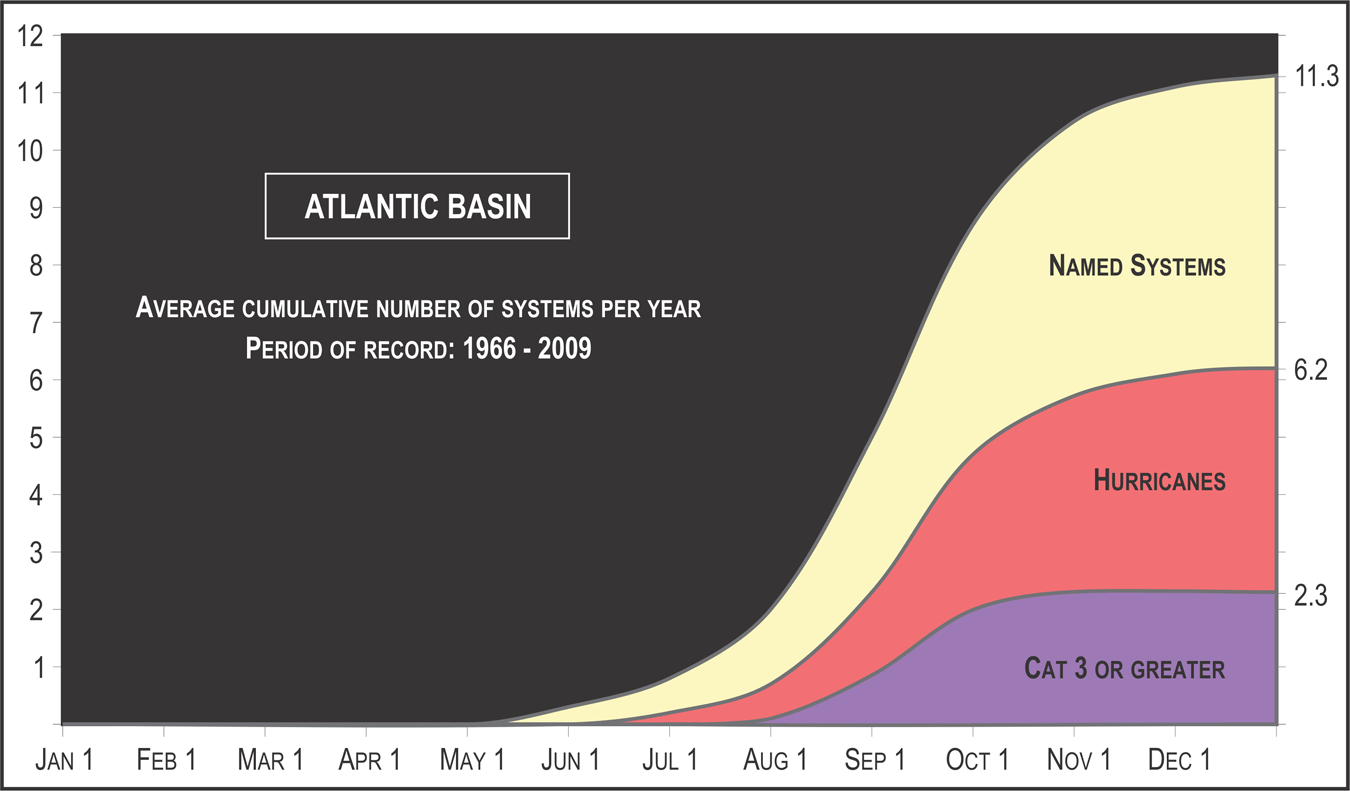
\includegraphics[width=0.7\textwidth]{img/cum-average-cat.png}
	\caption{Average cumulative number of storms in the Atlantic. Named systems are mostly tropical storms but can also be tropical depressions.\cite{climatology}}
	\label{fig:cat-climatology}
\end{figure}

Tropical cyclones rotate around a pressure minimum (the eye) which is enclosed by the eye wall. While the air is almost still in the eye, the maximum wind speeds is measured in the eye wall. The rotation around the center happens in different bands of updraft below the cloud that are alternated with rain bands. Finally, the warm core results in an anti-cyclonic outflow at the top of the storm. This structure is depicted in Fig.~\ref{fig:tc-structure} and together with the requirement of thermal wind balance leads to the characteristic warm core structure.
\begin{figure}[ht]
	\centering
	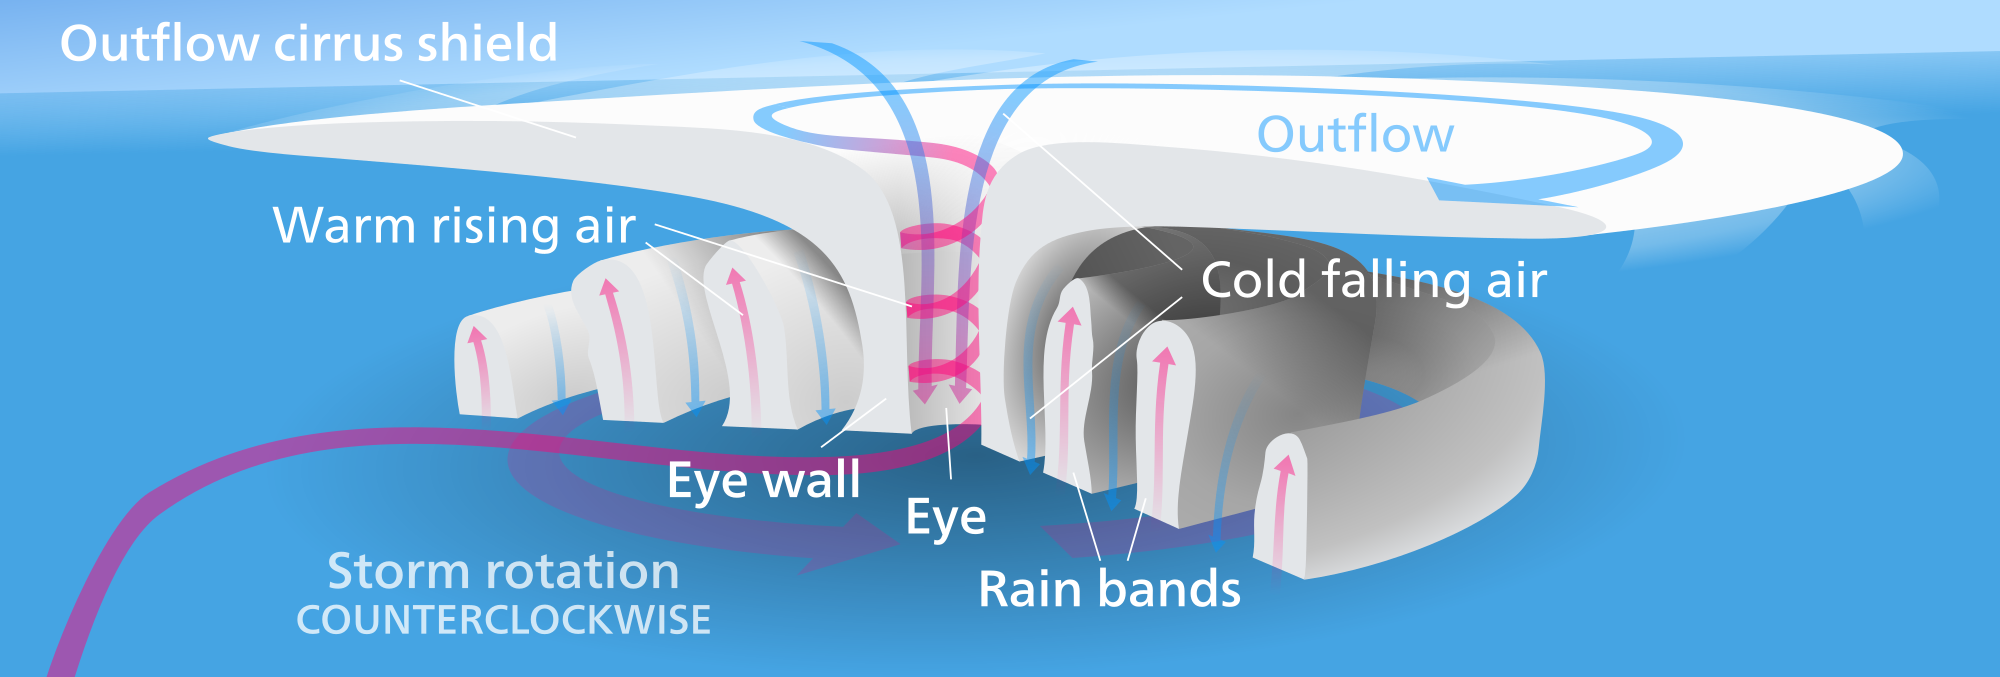
\includegraphics[width=0.8\textwidth]{img/hurricane-structure.png}
	\caption{Structure of a tropical cyclone in the Northern hemisphere~\cite{hurricane-structure}}
	\label{fig:tc-structure}
\end{figure}
In order for a storm to develop, a number of TC genesis criteria have to be met. Not all of them have to be satisfied but they do offer a good indicator for the probability of storm formation.
The criteria as summarised in \cite{lohmann-storms} are as follows:
\begin{itemize}
	\item sea surface temperature (SST) above 26.5\degree C to at least a depth of 50m
	\item sufficiently moist mid-troposphere for deep convection
	\item Appreciable moisture flux at the ocean-air interface to sustain a conditionally unstable thermodynamic environment \cite{moisture-flux}
	\item A distance of at least \unit[5]{\degree} from the equator, so that the Coriolis effect is strong enough to initiate the cyclone's rotation. \cite{coriolis}
	\item A pre-existing weather disturbance with sufficient vorticity and convergence, e.g. a tropical easterly wave.
	\item Low vertical wind shear between the surface and the upper troposphere
\end{itemize}


\section{Previous work on TC Tracking}\label{sec:tracking}
A large body of work exists on tracking meteorological phenomena. In this context tracking can be understood as following the same physical object in time.\newline
For instance an effort was conducted to compare different extratropical cyclone tracking algorithms in ~\cite{extratropical}. While extratropical cyclones differ significantly from tropical cyclones for example in regards to their occurrence frequency and physical structure, there are some common themes that apply to both tracking endeavours. The study found that the 15 compared algorithms disagree strongly on the total number of cyclones and the detection of weak cyclones, and agree best for stronger cyclones. It will be shown in Sec.~\ref{sec:results} of this report that these findings also apply to the tracking of TCs.\newline
Another work compared the predictions of two TC tracking schemes for several idealised climate simulations \cite{comp-climate-schemes}. The authors find a strong dependence of the results on the used parameter thresholds. They furthermore distinguish between algorithms using experimentally motivated parameter thresholds and those using deviations from the surrounding mean. They find that deviation conditions are more universal in respect to the climate model that they are applied to. The algorithm used in our report uses a mix of both types.\newline
The algorithm of this paper was inspired by the one in \cite{orig-tracking}. In the paper the authors discuss tracking of TCs in ERA-40 reanalysis data. The algorithm was adjusted for use with ICON data in the following ways: The sea level pressure (SLP) minimum criterion and vorticity threshold are retained. The original algorithm requires SLP minima to be \unit[250]{km} apart and to exhibit a minimum vorticity of \unit[5\times $10^{-5}$]{$s^{-1}$} (Equivalent to \textbf{slpdis} and \textbf{vormin} from Sec.~\ref{sec:tracking}). Furthermore, the vertical wind shear criterion is disregarded because TCs can also exist despite wind shear and the more definitive warm core criterion could be implemented to to the higher resolution of the ICON simulation. The minimum required lifetime is relaxed from 36 to 18 hours in the interest of tracking shorter-lived storms. Finally no special criterion over land is used but a minimum SST of \unit[24]{\degree C} required.